\documentclass{beamer}
\mode<presentation>

%%%%%%%%%%%%%%%%%%%%%%%%%%%%%%%%%%%%%%%%%%%%%%%%%%%%%%%%%%%%%%%%%%%%%%%%%%%%%
% preamble
\newtheorem{assumption}{Assumption}
\newtheorem{proposition}{Proposition}
\usepackage {mathtools}

\title{Counterfactual and  Synthetic Control Method: Causal Inference with Instrumented Principal Component Analysis}
\author{Cong Wang}
\institute{Sapienza University of Rome}
\date{\today}

\begin{document}

%%%%%%%%%%%%%%%%%%%%%%%%%%%%%%%%%%%%%%%%%%%%%%%%%%%%%%%%%%%%%%%%%%%%%%%%%%%%%
% title page
\begin{frame}
\titlepage
\end{frame}

%%%%%%%%%%%%%%%%%%%%%%%%%%%%%%%%%%%%%%%%%%%%%%%%%%%%%%%%%%%%%%%%%%%%%%%%%%%%%
% background and motivation
\begin{frame}{Background \& Motivation}
All the methods for causal inference can viewed as missing data imputation methods, where some are more explicit than others. -- \textcolor{blue}{Imbens and Rubin (2015)}.

\begin{itemize}
    \item Matching method explicity impute the missing counterfactual of trated $X_i$ by control $X_{j(i)}$.
    \item Difference-in-difference (DID) method implicitly impute the missing counterfactual by differencing the treated and controls before and after the treatment.
    \item Novel synthetic control method (SCM) explicitly impute the missing counterfactual of $Y_{it}$ with a weighted average of control units, without extrapolation.
    $$
    \hat{Y}_{it} = \sum_{j=1}^{J} W_{j} Y_{jt}
    $$
\end{itemize}

\end{frame}

%%%%%%%%%%%%%%%%%%%%%%%%%%%%%%%%%%%%%%%%%%%%%%%%%%%%%%%%%%%%%%%%%%%%%%%%%%%%%
% impute counterfactual by modeling the DGPs
\begin{frame}{Impute Counterfactual by Modeling the DGPs}
\begin{itemize}
    \item After transforming the causal inference problem into a missing data imputation problem, it is natural to think about modeling the data generating process (DGPs).
    \item Factor model is popular for its flexibility and sparsity in DGPs modeling. (\textcolor{blue}{Bai (2003)}, \textcolor{blue}{Stock and Watson (2002), etc.})
\end{itemize}

\textbf{A brief history of using the factor model for causal inference:}
\begin{enumerate}
    \item Pure factor models. \textcolor{blue}{Hsiao et al. (2012)} appear to be the first to use factor models for causal inference.
    $$y_{it} = \lambda_i F_t + \epsilon_{it}$$
    \item Interactive fixed effects model. \textcolor{blue}{Xu (2016)} use factor model plus regression terms.
    $$y_{it} = \lambda_{i} F_t + X_{it} \beta + \epsilon_{it}$$
\end{enumerate}
\end{frame}

%%%%%%%%%%%%%%%%%%%%%%%%%%%%%%%%%%%%%%%%%%%%%%%%%%%%%%%%%%%%%%%%%%%%%%%%%%%%%
% set up
\begin{frame}{Set up}
    \begin{itemize}
        \item $Y_{it}$ is the observed outcome for unit $i=1,2,\cdots, N$ at time $t=1,\cdots,T.$
        \item Total number of observed units is $N=N_{treat}+N_{ctrl},$ for $N_{ctrl}$ number of units in the control group $\mathcal{C}$ and $N_{treat}$ units in the treated group $\mathcal{T}$.
        \item Each unit is observed over $T=T_{pre}+T_{post}$ periods.
        \item Our target estimand is the average treatment effect for the treated units (ATT) in the post-treatment periods.
    \end{itemize}

\begin{assumption}
    Functional form:
    \begin{align*}
        & Y_{it} = D_{it}\circ \delta_{it} + \Lambda_{it}F'_t + \mu_{it} \\
        & \Lambda_{it} = X_{it}\Gamma + H_{it}
    \end{align*}
\end{assumption}
\end{frame}

\begin{frame}{Set up}
\begin{itemize}
    \item where $X_{it} = [x^1_{it}, \cdots, x^L_{it}]$ is a vector of observed covariates. $F_t = [f^1_t, \cdots, f^K_t]$ is a vector of unobserved time-varying factors. $\Lambda_{it} = [\lambda^1_{it}, \cdots, \lambda^K_{it}]$ is a vector of unobserved factor loading instrumented by covariates $X_{it}$.
    \item We use \textcolor{blue}{Neyman (1932)} and \textcolor{blue}{Rubin (2003)} potential outcome framework to specify the potential outcome for treated and control units:
\end{itemize}

\begin{equation*}
\begin{cases}
      Y_{it}^1 = \delta_{it} + X_{it} \Gamma F'_t + \epsilon_{it} & if \ i \in \mathcal{T} \ \& \ t > T_{pre} \\
      Y_{it}^0 = X_{it} \Gamma F'_t + \epsilon_{it} & otherwise.
\end{cases}
\end{equation*}
\end{frame}

%%%%%%%%%%%%%%%%%%%%%%%%%%%%%%%%%%%%%%%%%%%%%%%%%%%%%%%%%%%%%%%%%%%%%%%%%%%%%
% treatment assignment
\begin{frame}{Treatment Assignment}
\begin{itemize}
    \item To simplify the estimation, we focus on the block assignment scenario where all the treated units are treated at the same time 
    (can be relaxed) and the treatment once turned on can not be turned off.
\end{itemize}
\begin{figure}
    \centering
    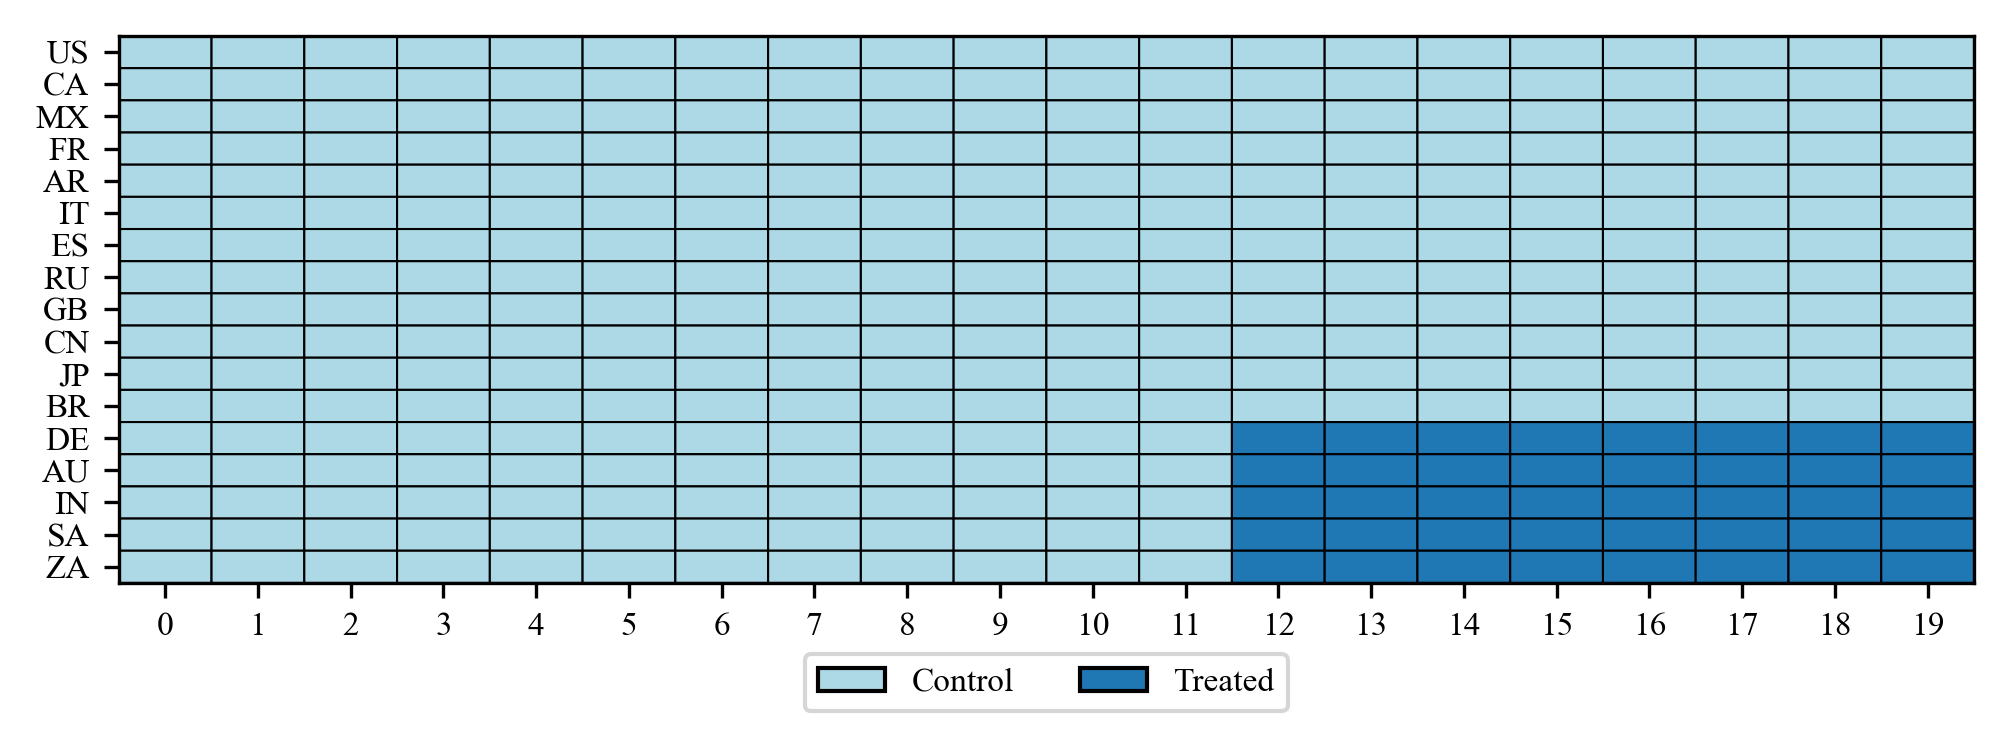
\includegraphics[width=0.8\textwidth]{figs/block_assignment.png}
    \caption{Block assignment scenario}
\end{figure}
\end{frame}

\begin{frame}{Treatment Assignment}
Staggered adoption: treatment status is assigned at different periods. 
\begin{figure}
    \centering
    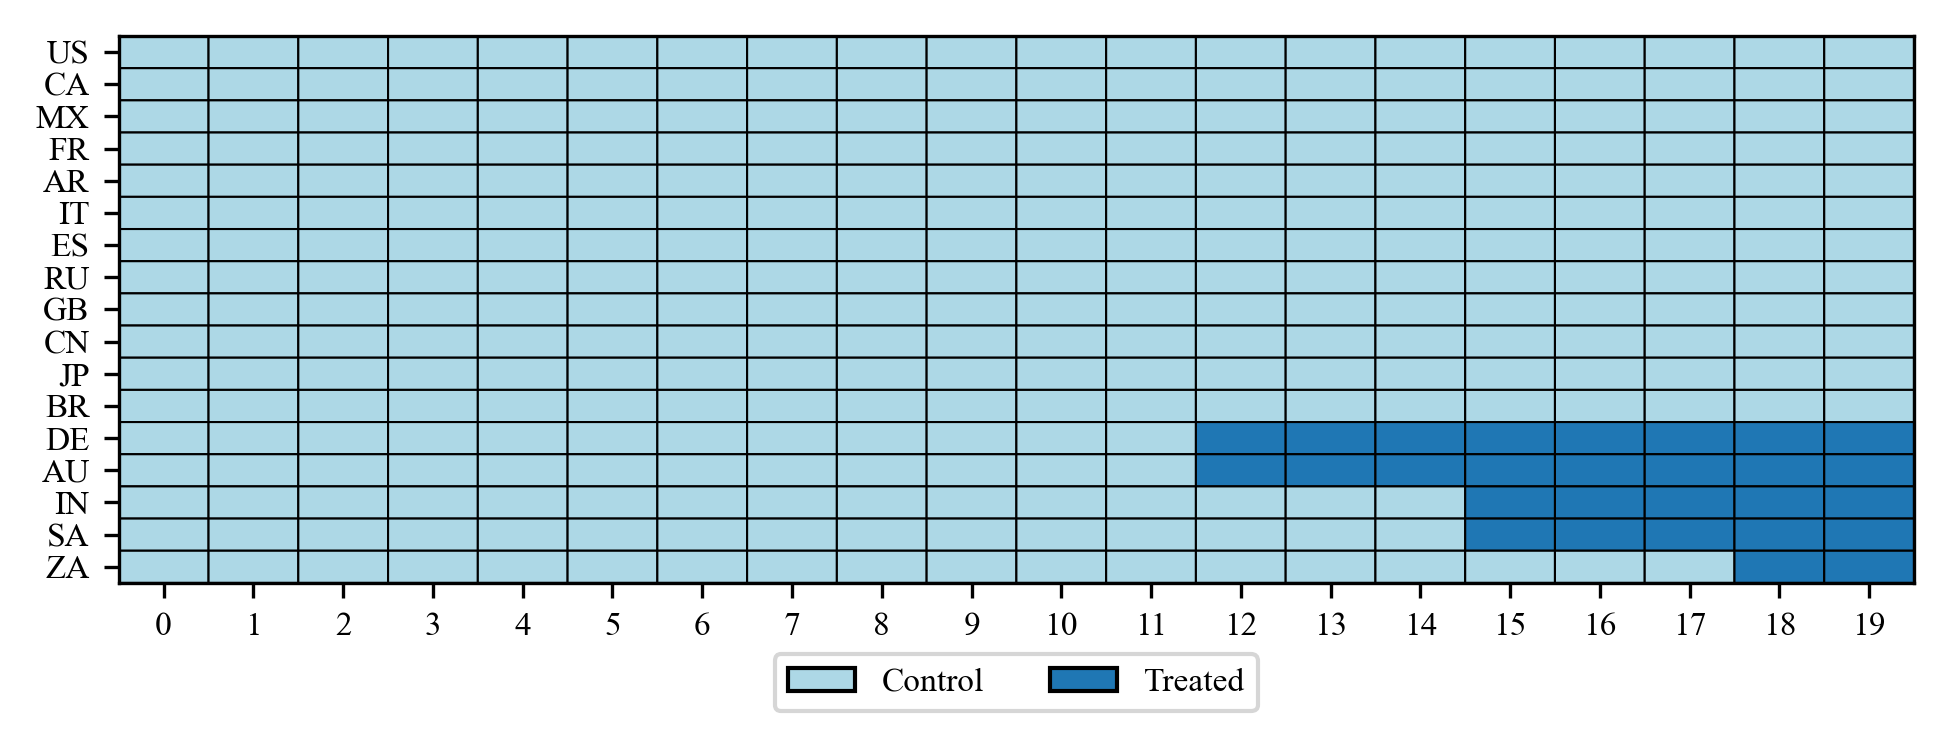
\includegraphics[scale=0.45]{figs/staggered_adoption.png}
\end{figure}  

Random assignment: treatment status is assigned randomly and it can be switched on and off multiple times. (Matrix completion \textcolor{blue}{Athey et al. (2021)})
\begin{figure}
    \centering
    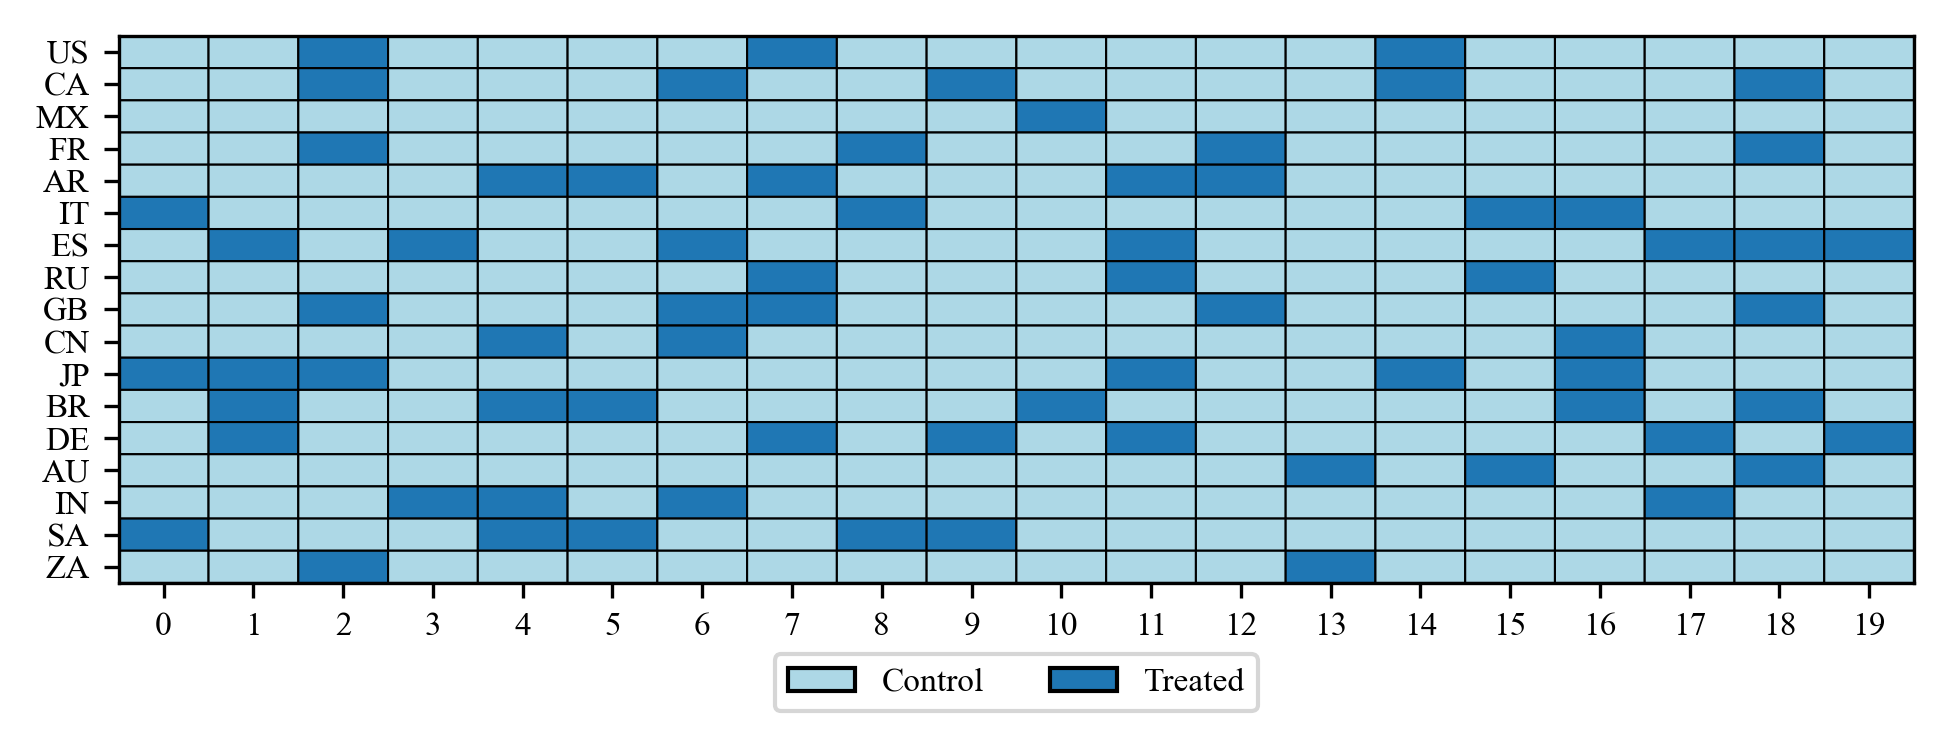
\includegraphics[scale=0.45]{figs/random_assignment.png}
\end{figure} 
\end{frame}

%%%%%%%%%%%%%%%%%%%%%%%%%%%%%%%%%%%%%%%%%%%%%%%%%%%%%%%%%%%%%%%%%%%%%%%%%%%%%
% Estimand
\begin{frame}{Estimand}
Under Nemany's potential outcome framework, our estimand ATT can be expressed as:
\begin{equation*}
    \widehat{ATT}_{t} = \frac{1}{N_{treat}}\sum_{i \in \mathcal{T}} \left( Y_{it}^1 - \hat{Y}_{it}^0 \right) = \frac{1}{N_{treat}}\sum_{i \in \mathcal{T}}\hat{\delta}_{it}.
\end{equation*}

\begin{figure}
    \centering
    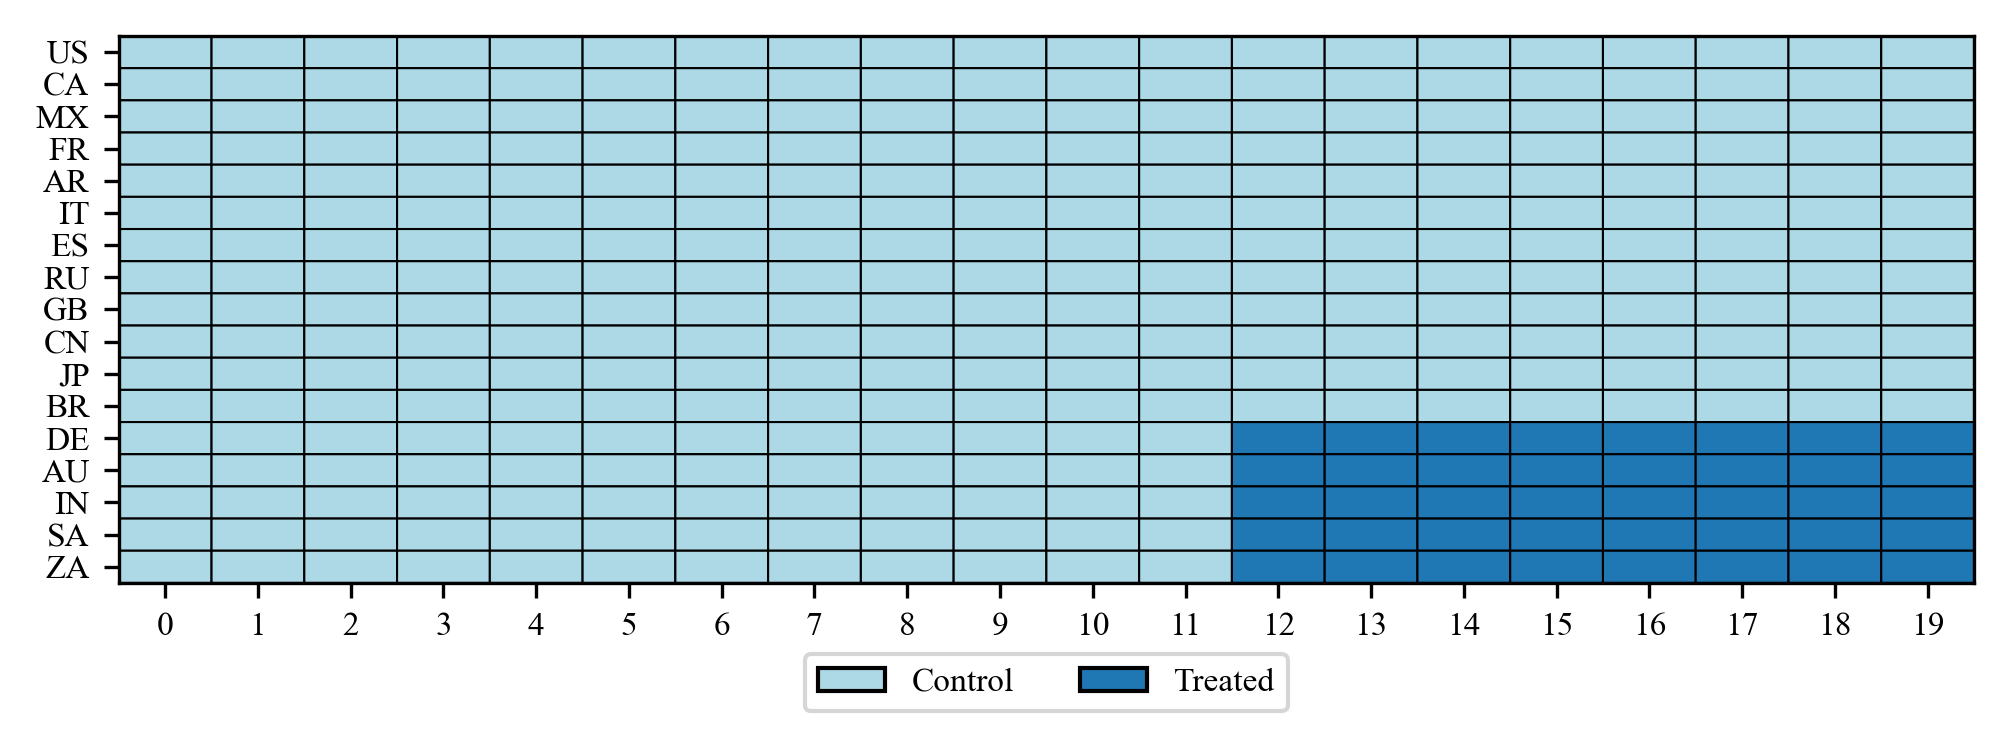
\includegraphics[scale=0.5]{figs/block_assignment.png}
\end{figure}
\end{frame}

%%%%%%%%%%%%%%%%%%%%%%%%%%%%%%%%%%%%%%%%%%%%%%%%%%%%%%%%%%%%%%%%%%%%%%%%%%%%%
% advantages of the CSC-IPCA method
\begin{frame}{Advantages of the CSC-IPCA Method}
    \begin{itemize}
        \item It incorporates the strengths of previous SCM approaches, such as the relaxation of the untestable parallel trends assumption (PTA).
        \item It complements the SCM method when targeted outcomes are outside the convex hull formulated by controls.
        \item It eliminates the need for correct model specification.
        \begin{enumerate}
            \item Estimates data with different DGPs other than the functional form, our method still excels.
            \item Covariates are incorporated into the model through a mapping matrix $\Gamma$ instead of a specific model specification.
        \end{enumerate}
    \end{itemize}
\end{frame}

\begin{frame}{Advantages of the CSC-IPCA Method}
    \begin{itemize}
        \item It inherits the ability of PCA to effectively handle high-dimensional data and enhances the value extracted from numerous covariates.
        \begin{enumerate}
            \item The mapping matrix $\Gamma$ conducts a dimensional reduction process, making it easier to handle high-dimensional financial data.
            \item Instrumented factor loadings $\Lambda_{it}$ inherit time-varying properties, making them more realistic in practice.
            \item Prediction information from covariates is more effectively handled. When there are unobserved covariates, this method is less biased compared to its peers.
        \end{enumerate}
    \end{itemize}
\end{frame}

%%%%%%%%%%%%%%%%%%%%%%%%%%%%%%%%%%%%%%%%%%%%%%%%%%%%%%%%%%%%%%%%%%%%%%%%%%%%%
% estimation
\begin{frame}{Estimation}
To combine the functional form we get the following structure component:
$$
Y_{it} = (X_{it}\Gamma) F'_{t} + \epsilon_{it}, \quad \epsilon_{it} = \mu_{it} + H_{it} F'_t.
$$
CSC-IPCA method is estimated by minimizing the sum of squared residuals of the following objective function:
$$
\underset{\Gamma, F_t}{\arg\min} \sum_{i} \sum_{t}\left( Y_{it} -(X_{it}\Gamma) F'_{t} \right)\left( Y_{it} - (X_{it}\Gamma) F'_{t}\right)'.
$$
\begin{itemize}
    \item Unlike PCA, the IPCA optimization challenge cannot be resolved through eigen decomposition.
    \item The optimization, as defined in the equation above, is quadratic with respect to either $\Gamma$ or $\boldsymbol{f}_t$, when the other is held constant.
    \item We can use alternating least squares (ALS) method for the numerical solution of this optimization problem.
\end{itemize}
\end{frame}

%%%%%%%%%%%%%%%%%%%%%%%%%%%%%%%%%%%%%%%%%%%%%%%%%%%%%%%%%%%%%%%%%%%%%%%%%%%%%
% estimation step 1
\begin{frame}{Estimation}
    \textbf{Step 1:} Estimate the time-varying factors $\hat{F}_t$ and the mapping matrix $\hat{\Gamma}_{\text{ctrl}}$ with an ALS algorithm, based exclusively on data from the control group for the whole time period.
    \begin{equation*}
    (\hat{\Gamma}_{ctrl}, \hat{F_t}) = \underset{\Gamma, F_t}{\arg\min} \sum_{i \in \mathcal{C}} \sum_{t \leq T}\left( Y_{it} - (X_{it}\Gamma) F'_{t} \right)\left( Y_{it} - (X_{it}\Gamma) F'_{t} \right)'.
    \end{equation*}
    
    With a fixed $\Gamma$, the solutions for $\boldsymbol{f}_t$ are t-separable and can be obtained via cross-sectional OLS for each $t$:
    
    \begin{equation*}
    \hat{\boldsymbol{f}}_t(\Gamma) = (\Gamma' X'_t X_t \Gamma)^{-1} \Gamma' X'_t Y_t.
    \end{equation*}
    
    Conversely, with known $\boldsymbol{f}_{t}$, the optimal $\Gamma$ (vectorized as $\boldsymbol{\gamma} = vect(\Gamma)$) is derived through pooled panel OLS of $y_{it}$ against $LK$ regressors, $\boldsymbol{x}_{it} \otimes \boldsymbol{f}_t$:
    
    \begin{equation*}
    \hat{\gamma} = \left( \sum_{i,t} (\boldsymbol{x}_{it}' \otimes \boldsymbol{f}_t) (\boldsymbol{x}_{it} \otimes \boldsymbol{f}_t') \right)^{-1} \left( \sum_{i,t} (\boldsymbol{x}_{it}' \otimes \boldsymbol{f}_t) y_{it} \right).
    \end{equation*}
\end{frame}

%%%%%%%%%%%%%%%%%%%%%%%%%%%%%%%%%%%%%%%%%%%%%%%%%%%%%%%%%%%%%%%%%%%%%%%%%%%%%
% estimation step 2
\begin{frame}{Estimation}
    \textbf{Step 2:} Estimate the mapping matrix $\hat{\Gamma}_{treat}$ for treated unit $i$ at time $t$, employing the previously estimated time-varying factors $\hat{F}_t$ and the observed covariates $X_{it}$, using only pretreatment data from the treated units.
    \begin{equation*}
    \hat{\Gamma}_{treat} = \underset{\Gamma}{\arg\min} \sum_{i \in \mathcal{T}} \sum_{t \leq T_{pre}} \left( Y_{it} - (X_{it} \Gamma) \hat{F}'_{t} \right) \left( Y_{it} - (X_{it} \Gamma) \hat{F}'_{t} \right)'.
    \end{equation*}
    
    The $\Gamma_{treat}$ is estimated through:
    \begin{equation*}
        \hat{\gamma} = \left( \sum_{i,t} (\boldsymbol{x}_{it}' \otimes \boldsymbol{f}_t) (\boldsymbol{x}_{it} \otimes \boldsymbol{f}_t') \right)^{-1} \left( \sum_{i,t} (\boldsymbol{x}_{it}' \otimes \boldsymbol{f}_t) y_{it} \right).
    \end{equation*}
    $$for \ i \in \mathcal{T}, T<= T_{pre}.$$
\end{frame}

%%%%%%%%%%%%%%%%%%%%%%%%%%%%%%%%%%%%%%%%%%%%%%%%%%%%%%%%%%%%%%%%%%%%%%%%%%%%%
% estimation step 3
\begin{frame}{Estimation}
    \begin{itemize}
        \item The estimation of $\boldsymbol{f}_{t}$ and $\Gamma$ is not deterministic.
        \item We can find any arbitrary rotation matrix $R$, such that $\boldsymbol{x}_{it}\Gamma R R^{-1}\boldsymbol{f}'_{t}$ yields the same structural component.
        \item We put specific constraints on the mapping matrix $\Gamma_{norm} = \Gamma_{treat}R$ and factor $\boldsymbol{f}_{norm} = R^{-1}\boldsymbol{f}_t$ for identification.
    \end{itemize}
\end{frame}

\begin{frame}{Estimation}    
    \textbf{Step 3:} The third step includes normalizing the estimated mapping matrix $\hat{\Gamma}_{treat}$ and $\hat{F_t}$ by a set of constraints:
    
    \begin{equation*}
    \begin{aligned}
    \Gamma_{norm} &= \hat{\Gamma}_{treat} R, \\
    F_{norm} &= R^{-1} \hat{F}_t, \\
    s.t. \Gamma_{norm}'\Gamma_{norm} &= \mathcal{I}_K, \quad F_{norm} F_{norm}'/T = \text{Diagonal}.
    \end{aligned}
    \end{equation*}
    
    \begin{enumerate}
        \item Cholesky decomposition to get a upper triangular matrix $R_1 = cholesky(\Gamma' \Gamma)$,
        \item Singular value decomposition on $R_1\boldsymbol{f}_t\boldsymbol{f}_t'R_1'$ to get $R_2 = U$ where $U\Sigma V'=svd(R_1\boldsymbol{f}_t\boldsymbol{f}_t'R_1')$.
        \item Finally, the rotation matrix $R$ is given by: $R = R_1^{-1}R_2.$
        \end{enumerate}
\end{frame}

%%%%%%%%%%%%%%%%%%%%%%%%%%%%%%%%%%%%%%%%%%%%%%%%%%%%%%%%%%%%%%%%%%%%%%%%%%%%%
% estimation step 4
\begin{frame}{Estimation}
    \textbf{Step 4:} The final step involves imputing the counterfactual outcome $\hat{Y}_{it}^0$ for treated unit $i$ at time $t$ by substituting the estimated mapping matrix $\hat{\Gamma}_{norm}$ and the time varying factors $\hat{F}_{norm}$ into the following equation:
    
    \begin{equation*}
    \hat{Y}_{it}(0) = (X_{it} \hat{\Gamma}_{norm}) \hat{F}'_{norm}, \quad \forall i \in \mathcal{T}, \quad \& \quad T_{pre} < t \leq T.
    \end{equation*}    
    
    The estimated average treatment effect for treated is:
    \begin{equation*}
        \widehat{ATT}_{t} = \frac{1}{N_{treat}}\sum_{i \in \mathcal{T}} \left( Y_{it}^1 - \hat{Y}_{it}^0 \right) = \frac{1}{N_{treat}}\sum_{i \in \mathcal{T}}\hat{\delta}_{it}.
    \end{equation*}
\end{frame}

%%%%%%%%%%%%%%%%%%%%%%%%%%%%%%%%%%%%%%%%%%%%%%%%%%%%%%%%%%%%%%%%%%%%%%%%%%%%%
% hyperparameters tunning
\begin{frame}{Hyperparameter tuning}
\begin{figure}
    \centering
    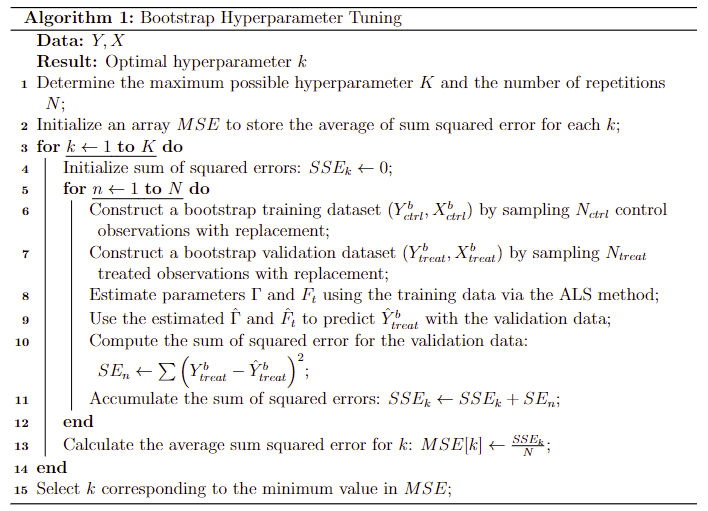
\includegraphics[scale=0.8]{figs/boots_tuning.png}
\end{figure}
\end{frame}

\begin{frame}{Hyperparameter tuning}
\begin{figure}
    \centering
    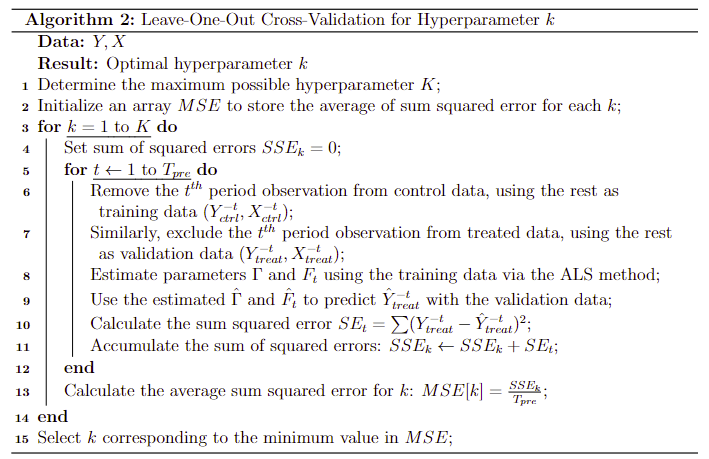
\includegraphics[scale=0.8]{figs/cv_tuning.png}
\end{figure}
\end{frame}

%%%%%%%%%%%%%%%%%%%%%%%%%%%%%%%%%%%%%%%%%%%%%%%%%%%%%%%%%%%%%%%%%%%%%%%%%%%%%
% inference

\begin{frame}{Inference}
We use conformal inference (\textcolor{blue}{Chernozhukov et al. (2021)}) to construct the confidence interval.

\begin{enumerate}
    \item We postulate a sharp null hypothesis, $H_0: \theta_{it} = \theta_{it}^0$. Under this null hypothesis, we adjust the outcome for treated units post-treatment as $\tilde{Y}_{it} = Y_{it} - \theta_{it}$.
    \item Following the estimation procedure to estimate the time-varying factor $F_t$ with only control data as before, and update the $\Gamma$ for the newly adjusted treated units with the \textbf{entire set of treated units}.
    \item Estimate the treatment effect and compute the residuals for the treated units in the post treatment period. The test statistic showing how large the residual is under the null:
    \begin{equation*}
    S(\hat{\mu}) = \left(\frac{1}{\sqrt{T_{post}}}\sum_{t > T_{pre}} |\hat{\mu}|^q \right)
    \end{equation*}
\end{enumerate}
\end{frame}

\begin{frame}{Inference}
\begin{enumerate}
\setcounter{enumi}{3}
    \item We employ $q=1$ for the permanent intervention effect as designed in our study.
    \item Block permute the residuals and calculate the test statistic in each permutation. The P-value is defined as:
    \begin{equation*}
    \hat{p} = 1 - \hat{F}(S(\hat{u})), \text{ where } \hat{F}(x) = \frac{1}{|\Pi|} \sum_{\pi \in \Pi} 1\{S(\hat{u}_\pi) < x\}.
    \end{equation*}
    \item Repeat the above procedures with different nulls to get different P-values and construct confidence intervals at different significance levels.
\end{enumerate}
\end{frame}

%%%%%%%%%%%%%%%%%%%%%%%%%%%%%%%%%%%%%%%%%%%%%%%%%%%%%%%%%%%%%%%%%%%%%%%%%%%%%
% simulation
\begin{frame}{Simulation}
We use the following DGPs to simulate the data:
$$
Y_{it} = D_{i} \delta'_{t} + X_{it}\beta' + (X_{it}\Gamma) F'_{t} + \alpha_i + \xi_t + \epsilon_{it}.
$$

\begin{itemize}
    \item $L=10$ and $K=3$.
    \item $X_{it} = [x_{it}^1, \ldots, x_{it}^{L}]$ denotes a vector of $L \times 1$ time-varying covariates, which follows a VAR(1) process. $X_{it} = \mu_i + A_i X_{i,t-1} + \nu_{it}$, where $A_i$ is a $ L \times L$ variance-covariance matrix.
    \item $F_t = [f_t^1, \ldots, f_t^3]$ denotes the vector of time-varying common factors, adhering to a similar VAR(1) process.
    \item The coefficient vector $\beta = [\beta^1, \ldots, \beta^{L}]$ associated with the covariates is drawn uniformly from $(0,1)$. 
    \item $\Gamma$, the $L \times K$ mapping matrix for the factor loadings, is drawn uniformly from $(-0.1, 0.1)$.
    \item The treatment indicator $D_{it}$ is binary. The heterogeneous treatment effect is modeled as $\delta_{it} = \bar{\delta}_{it} + e_{it}$. $\bar{\delta_t} = [0, \cdots, 0, 1,2,\ldots,T_{post}]$ represents a time-varying treatment effect.
\end{itemize}
\end{frame}

\begin{frame}{Simulation}
\begin{itemize}
    \item There is a possibility that treated units are not in the convex hull formulated by controls.
    \item From the simple event study plot, the parallel trend assumption is not satisfied.
\end{itemize}
\begin{figure}
    \centering
    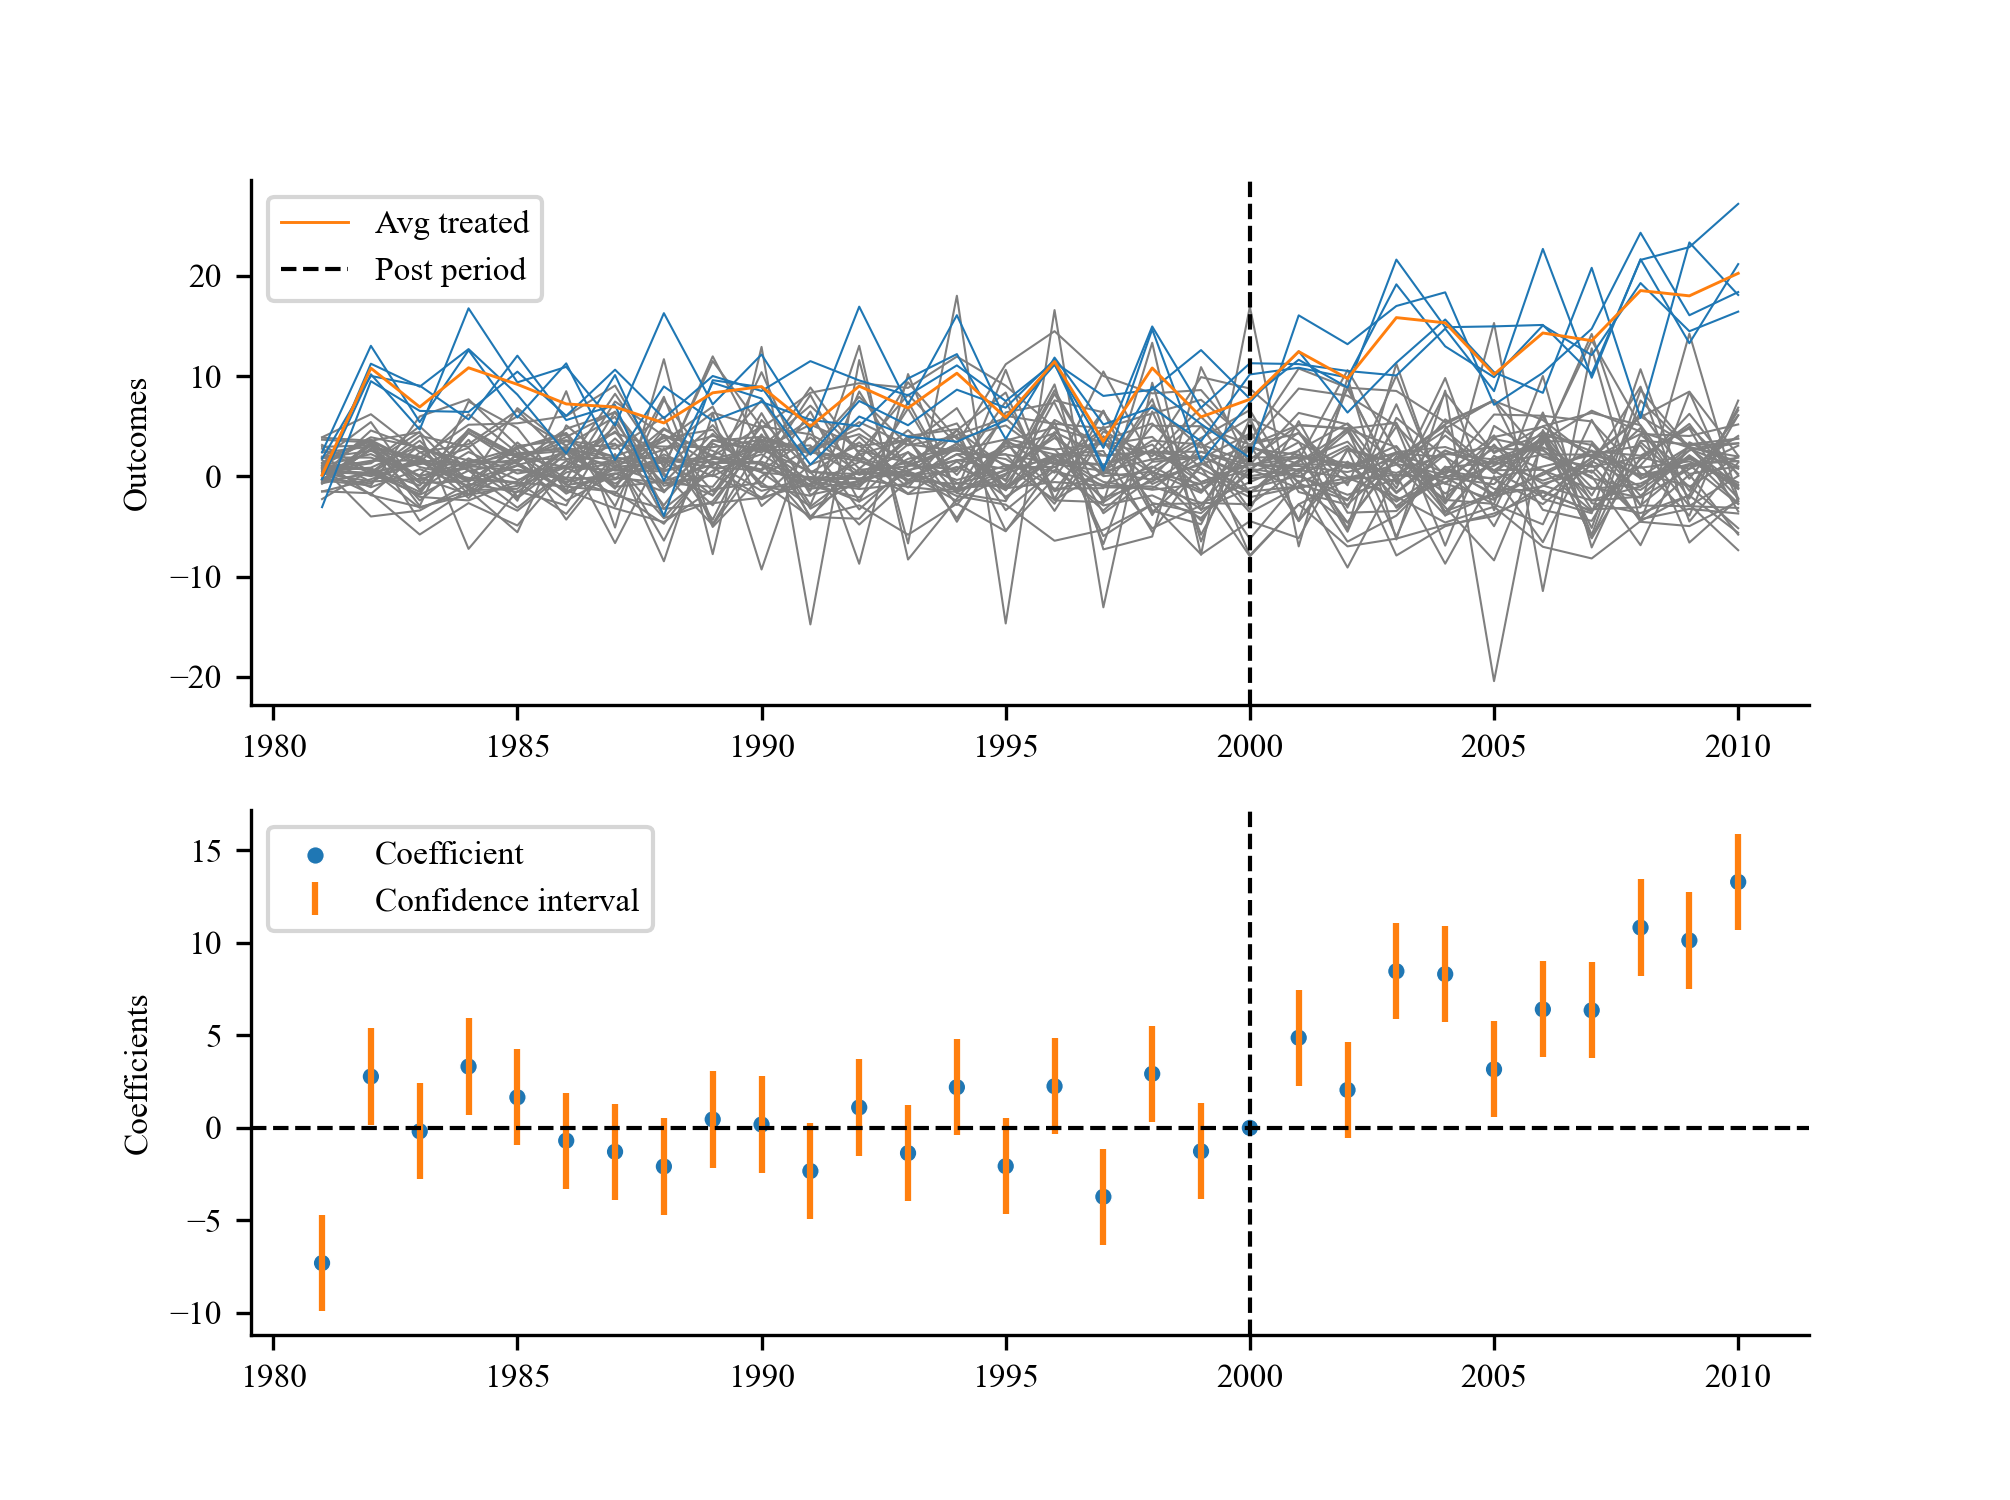
\includegraphics[scale=0.5]{figs/data_plot.png}
\end{figure}
\end{frame}

\begin{frame}{An example}
\begin{itemize}
    \item The upper panel shows the average synthetic control's outcome perfectly overlaps with the actual average treated outcome before the treatment.
    \item The lower panel shows the average treatment effect before and after treatment with a 90\% confidence interval.
\end{itemize}
\begin{figure}
    \centering
    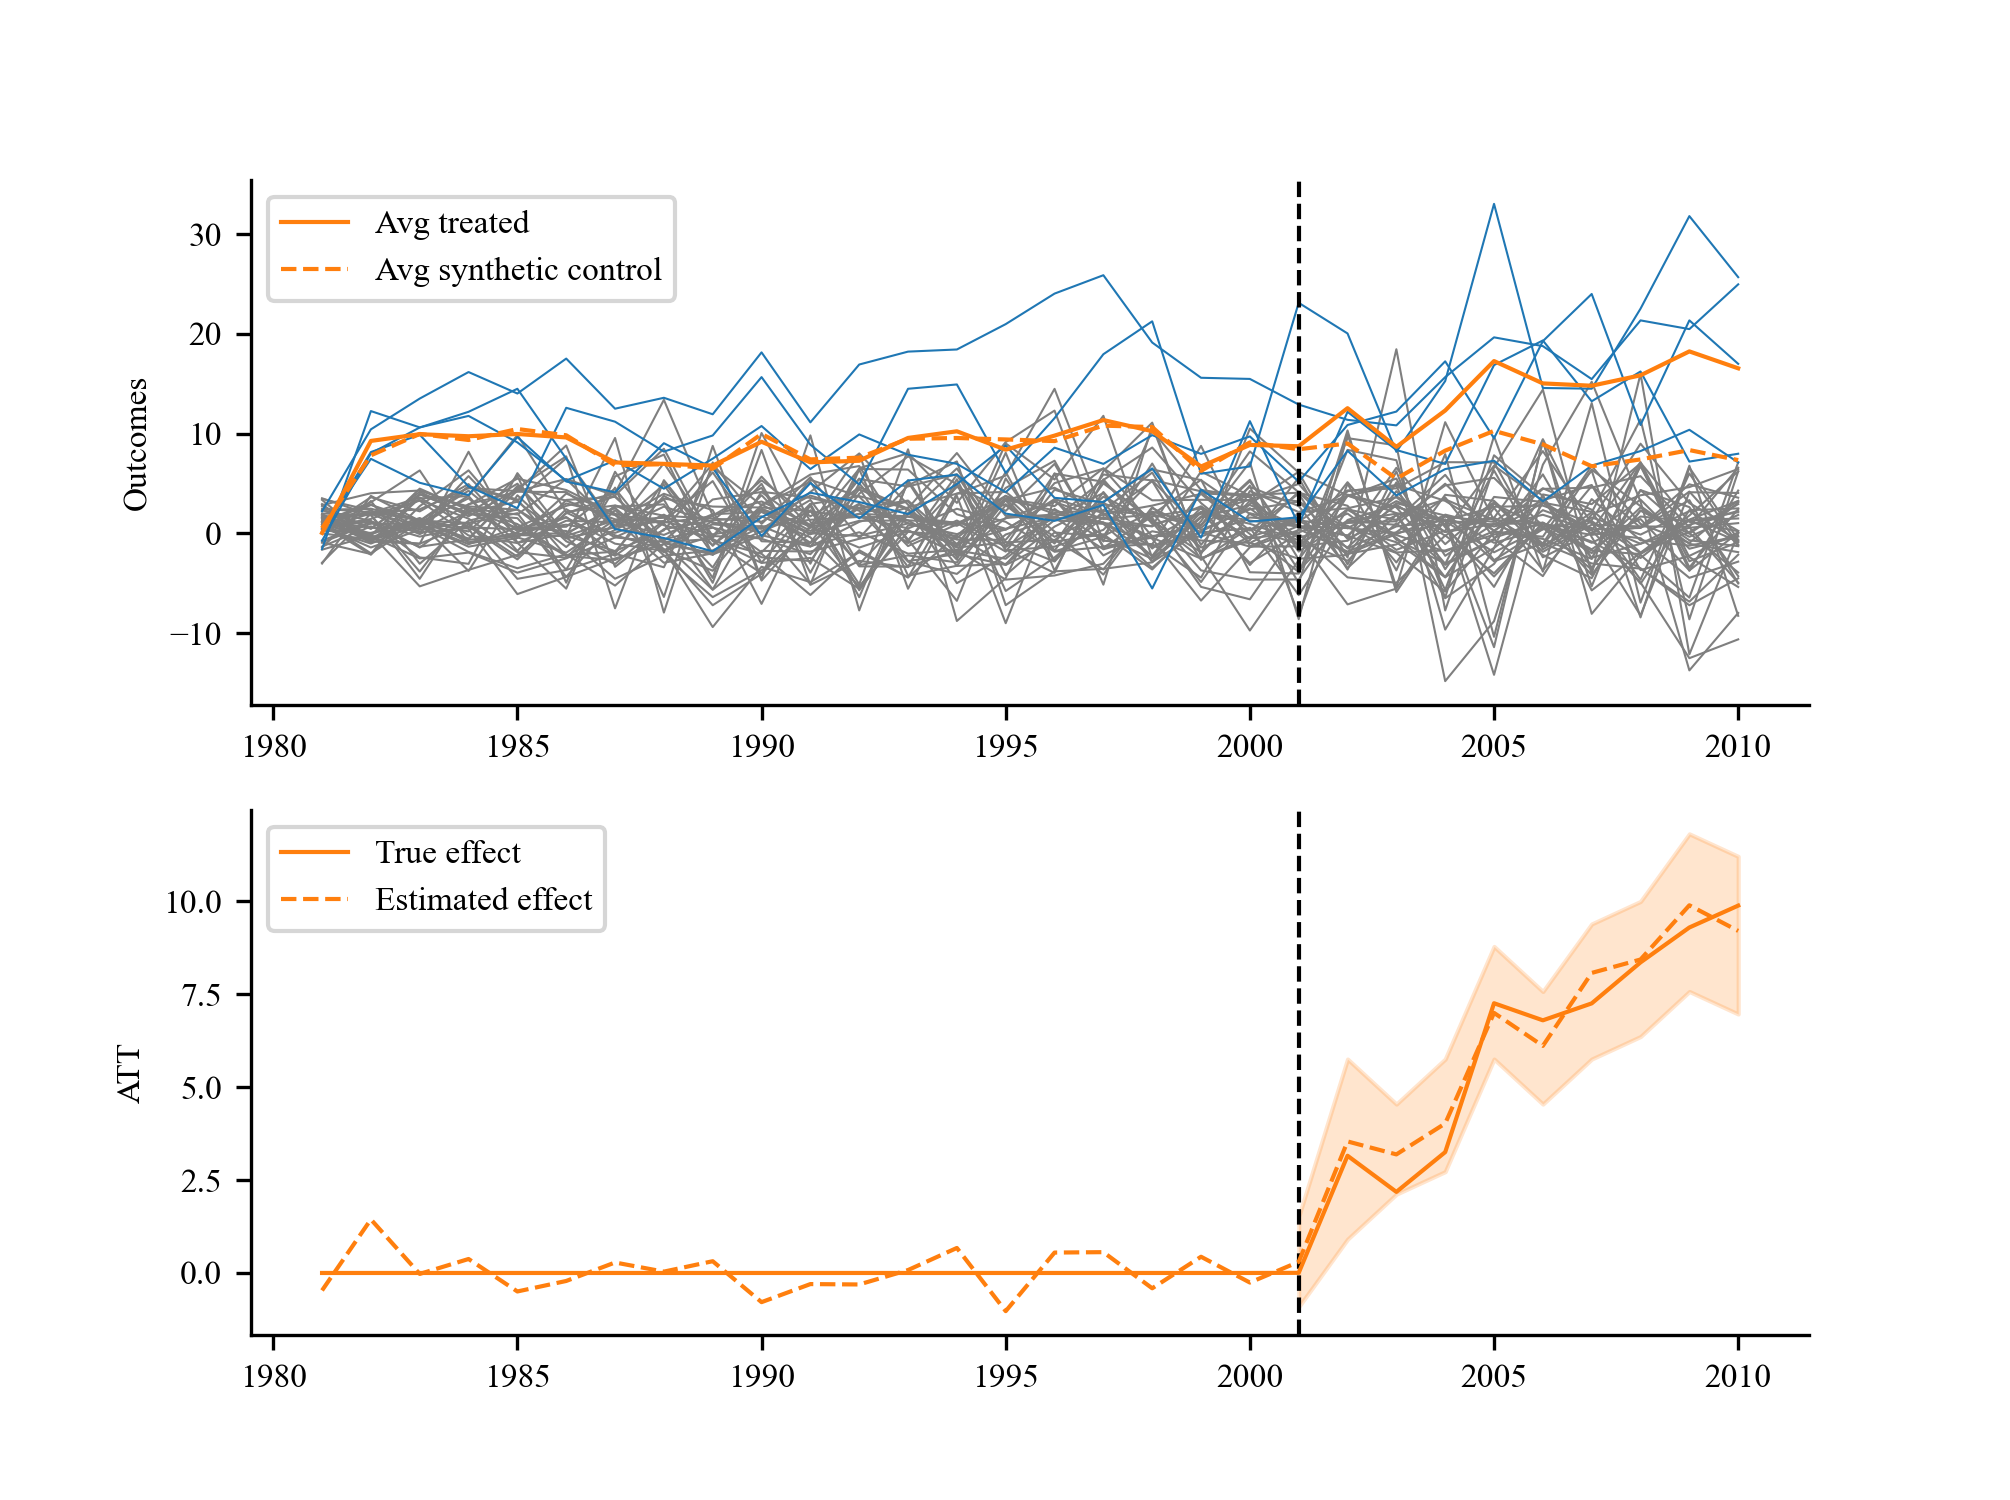
\includegraphics[scale=0.5]{figs/estimation.png}
\end{figure}
\end{frame}

%%%%%%%%%%%%%%%%%%%%%%%%%%%%%%%%%%%%%%%%%%%%%%%%%%%%%%%%%%%%%%%%%%%%%%%%%%%%%
% bias comparison
\begin{frame}{Bias comparison}
\begin{itemize}
    \item When all covariates are observed, both CSC-IPCA and CSC-IFE demonstrate unbiasedness and effectively estimate the true ATT.
    \item SCM exhibits an upward bias for the poor pre-treatment fit.
    \item As the number of unobserved covariates increases, both CSC-IPCA and CSC-IFE lose efficiency, but the CSC-IPCA estimator remains less unbiased than CSC-IPCA estimator.
\end{itemize}
\begin{figure}
    \centering
    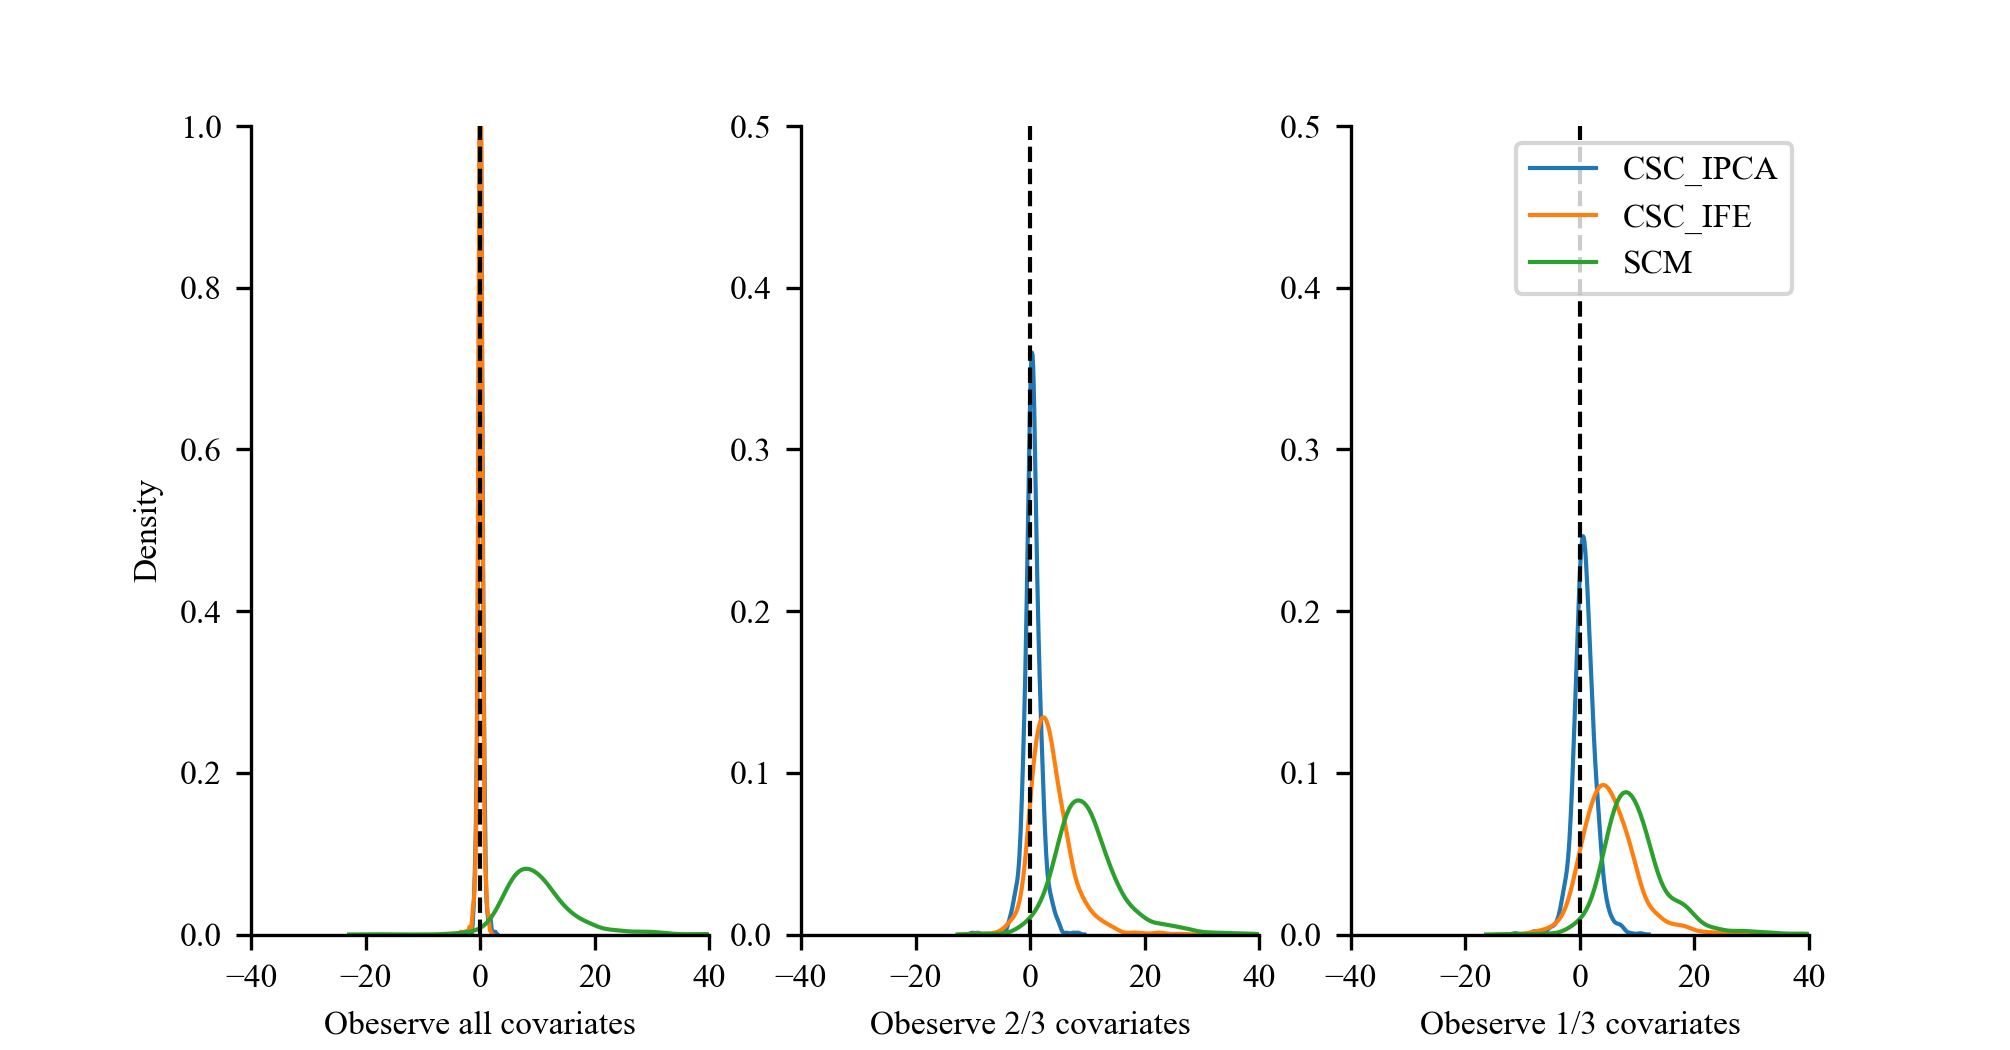
\includegraphics[scale=0.5]{figs/bias_compar1.png}
\end{figure}
\end{frame}

%%%%%%%%%%%%%%%%%%%%%%%%%%%%%%%%%%%%%%%%%%%%%%%%%%%%%%%%%%%%%%%%%%%%%%%%%%%%%
% finite sample performance
\begin{frame}{Finite sample property}
\begin{itemize}
    \item The bias, RMSE, and STD are estimated based on 1000 simulations.
    \item $N_{treat} = 5, T_{post}=5, L=10$. We vary the number of control units $N_{ctrl}$, pre-treatment period $T_{pre}$, and the proportion of observed covariates $\alpha$.
    \item The convergence rate of the CSC-IPCA estimator is the smaller one of $\mathcal{O}_p\left(\sqrt{N_{ctrl}}\right)$ and $\mathcal{O}_p\left(\sqrt{N_{treat}T_{pre}}\right)$.
\end{itemize}
\begin{figure}
    \centering
    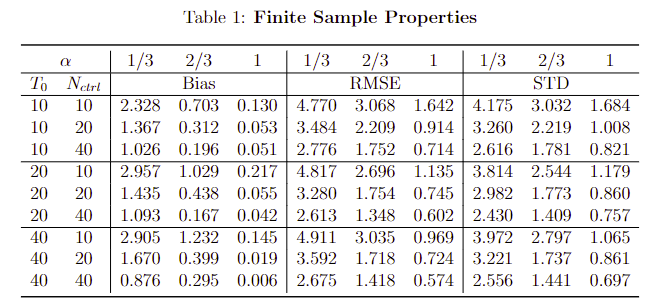
\includegraphics[scale=0.8]{figs/finite_sample.png}
\end{figure}
\end{frame}

%%%%%%%%%%%%%%%%%%%%%%%%%%%%%%%%%%%%%%%%%%%%%%%%%%%%%%%%%%%%%%%%%%%%%%%%%%%%%
% identification assumption
\begin{frame}{Identification assumptions}
\begin{assumption}
Assumption for consistency:
\begin{enumerate}
    \item Covariate orthogonality: $E\left[\textbf{x}'_{it} \epsilon_{it}\right] = \textbf{0}_{L\times 1}$,
    
    \item The following moments exist: $\mathrm{E}\|\boldsymbol{f}_{t}\boldsymbol{f}'_{t}\|^2$, $\mathrm{E}\|\boldsymbol{x}'_{it}\epsilon_{it}\|^2$, $\mathrm{E}\|\boldsymbol{x}'_{it}\boldsymbol{x}_{it}\|^2$, $\mathrm{E}\left[\|\boldsymbol{x}'_{it}\boldsymbol{x}_{it}\|^2\|\boldsymbol{f}_{t}\boldsymbol{f}'_{t}\|^2 \right]$, 
    
    \item The parameter space $\Psi$ of $\Gamma$ is compact and away from rank deficient: $\det{\Gamma' \Gamma} > \epsilon$ for some $\epsilon>0$,
    
    \item Almost surely, $\boldsymbol{x}_{it}$ is bounded, and define $\Omega_t^{xx} := \mathrm{E}\left[ \boldsymbol{x}_{it}' \boldsymbol{x}_{it} \right]$, then almost surely, $\Omega_t^{xx} > \epsilon$ for some $\epsilon > 0$.
\end{enumerate}
\end{assumption}
\end{frame}

\begin{frame}{Identification assumption}
\begin{assumption}
Assumptions for asymptotic normality:
\begin{enumerate}
    \item $\text{As } N, T \to \infty, \: \frac{1}{\sqrt{NT}} \sum_{i,t} \text{vect}\left( \boldsymbol{x}'_{it} \epsilon_{it} \boldsymbol{f}'_{t} \right) \xrightarrow{d} \text{Normal} \left(0, \Omega^{x\epsilon f} \right)$,
    
    \item $\text{As } N \to \infty, \: \frac{1}{\sqrt{N}} \sum_{i} \text{vect}\left( X'_{i} \epsilon_{i} \right) \xrightarrow{d} \text{Normal} \left(0, \Omega^{x\epsilon} \right) \: \text{for} \: \forall t$,
    
    \item $\text{As } N, T \to \infty, \: \frac{1}{\sqrt{T}} \sum_{t} \text{vect}\left( \boldsymbol{f}_{t}\boldsymbol{f}'_{t} - \mathrm{E}[\boldsymbol{f}_{t}\boldsymbol{f}'_{t}] \right) \xrightarrow{d} \text{Normal} \left(0, \Omega^{f} \right)$.
    
    \item Bounded dependence: $\frac{1}{NT} \sum_{i,j,t,s}\|\tau_{ij, ts}\| < \infty$, where $\tau_{ij, ts} := \mathrm{E} \left[ \boldsymbol{x}'_{it} \epsilon_{it} \epsilon'_{js} \boldsymbol{x}_{js} \right]$
    
    \item Constant second moments of the covariates: $\Omega_t^{xx} = \mathrm{E}\left[ X_{t} X'_{t} \right]$ is constant across time periods.
    \end{enumerate}
\end{assumption}
\end{frame}

%%%%%%%%%%%%%%%%%%%%%%%%%%%%%%%%%%%%%%%%%%%%%%%%%%%%%%%%%%%%%%%%%%%%%%%%%%%%%
% formal results
\begin{frame}{Formal result}
we can formulate a target function for $\Gamma$ as follows:
\begin{equation*}
\label{eqn: target}
G(\Gamma) = \frac{1}{2NT}\sum_{i,t} \left( y_{it} - \boldsymbol{x}_{it}\Gamma \boldsymbol{\hat{f}}_t \right)^2.
\end{equation*}
The Hessian matrix $H(\Gamma)$ is defined as the second derivative of the target function $G(\Gamma)$ with respect to $\Gamma$: $H(\Gamma) = \frac{\partial^2 G(\Gamma)}{\partial \Gamma \partial \Gamma'}$. 

To satisfy the normalization criteria, we define the following identification function:
\begin{equation*}
\label{eqn: identification}
I(\Gamma) := \begin{bmatrix}
    \text{veca}(\Gamma' \Gamma - \mathcal{I}_K) \\
    \text{vecb}\left(\frac{1}{T} \sum_{t} \boldsymbol{\hat{f}}_t\boldsymbol{\hat{f}}_t' - V^{ff}\right)
    \end{bmatrix}
\end{equation*}
where $V^{ff} = E\left[\boldsymbol{f}_t\boldsymbol{f}'_t\right]$, meanwhile, $\text{veca}(\cdot)$ and $\text{vecb}(\cdot)$ vectorize the upper triangular entries of a square matrix.

The Jacobian matrix $J(\Gamma)$ as the derivative of the identification function $I(\Gamma)$ with respect to $\Gamma$: $J(\Gamma) = \frac{\partial I(\Gamma)}{\partial \Gamma}$.
\end{frame}

\begin{frame}{Formal result}
\begin{proposition}
\label{prop: gamma}
Under the above assumptions, mapping matrix estimation error centered against the normalized true mapping matrix converges to a normal distribution at the rate of $\sqrt{NT}$: as $N, T \rightarrow \infty$ such that $T/N \rightarrow \infty$,

$$
\sqrt{NT} \left( \hat{\boldsymbol{\gamma}} - \boldsymbol{\gamma}^0 \right) \xrightarrow{d} - \left( H^{0'}H^0 + J^{0'}J^0 \right)^{-1}H^{0'}Normal(0, \mathbb{V}^{[1]})
$$
\end{proposition}
where $H^0:= \frac{\partial S(\Gamma)}{\partial \boldsymbol{\gamma}}|_{\boldsymbol{\gamma} = \boldsymbol{\gamma}^0}$ and $J^0:= \frac{\partial I(\Gamma)}{\partial \boldsymbol{\gamma}}|_{\boldsymbol{\gamma} = \boldsymbol{\gamma}^0}$, $\mathbb{V}^{[1]} = \left( Q^0 \otimes \mathcal{I}_K \right) \Omega^{x\epsilon f} \left( Q^{0'} \otimes \mathcal{I}_K \right)$, and $Q^0 := Q_t(\Gamma^0)$ given that $Q_t(\Gamma) := \mathcal{I}_L - \Omega_t^{xx} \left( \Gamma' \Omega^{xx}_t \Gamma \right)^{-1}\Gamma'$ is constant over $t$ under the normality assumption.
\end{frame}

\begin{frame}{Formal result}
\footnotesize
    \begin{proposition}
\label{prop: factor}
Under the Assumptions, factor estimation error centered against the normalized true factor converges to a normal distribution at the rate of $\sqrt{N}$: as $N, T \to \infty$ for $\forall t$,
$$
\sqrt{N}\left(\hat{\boldsymbol{f}}_t - \boldsymbol{f}^0_t\right) \xrightarrow{d} N\left(0, \mathbb{V}_t^{[2]}\right),
$$
\end{proposition}

\textbf{Proof:} Decompose the left-hand side equation:
\begin{equation*}
\begin{aligned}
\sqrt{N}\left(\boldsymbol{\hat{f}}_t - \boldsymbol{f}_t\right) &= \sqrt{N}\left(\left( \hat{\Gamma}'X'_tX_t\hat{\Gamma} \right)^{-1}\hat{\Gamma}'X_t' \left(X_t\hat{\Gamma}\boldsymbol{f}_t+ \boldsymbol{\tilde{\epsilon}}_t \right) - \boldsymbol{f}_t\right)\\
&= \sqrt{N}\left(\left( \hat{\Gamma}'X'_tX_t\hat{\Gamma} \right)^{-1}\hat{\Gamma}'X_t' \left(X_t \hat{\Gamma}\boldsymbol{f}_t\right) - \boldsymbol{f}_t\right) + \sqrt{N}\left( \hat{\Gamma}'X'_tX_t\hat{\Gamma} \right)^{-1}\hat{\Gamma}'X_t'\boldsymbol{\tilde{\epsilon}}_t
\end{aligned}
\end{equation*}
where $\tilde{\epsilon}_t$ is the estimated error term with estimated $\Gamma$ and true $\boldsymbol{f}_t$. Given Proposition \ref{prop: gamma}, $\hat{\Gamma} - \hat{\Gamma}^0 = \mathcal{O}_p \left( 1/\sqrt{NT} \right)$. The first term is simply $\mathcal{O}_p\left(1/\sqrt{NT}\right)$. For the second term:

\begin{equation*}
\begin{aligned}
\sqrt{N}\left( \hat{\Gamma}'X'_tX_t\hat{\Gamma} \right)^{-1}\hat{\Gamma}'X_t'\boldsymbol{\epsilon}_t = &\sqrt{N}\left( \Gamma'X'_tX_t\Gamma \right)^{-1}\Gamma'X_t'\boldsymbol{\epsilon_t} + \mathcal{O}_p(1) \\
& \xrightarrow{d} Normal(0, \mathbb{V}_t^{[2]})
\end{aligned}
\end{equation*}
\end{frame}

\begin{frame}{Formal result}
\footnotesize
\begin{theorem}
\label{thm: bias}
Under Assumptions, the CSC-IPCA estimator $\mathrm{E}\left(\widehat{ATT}_{t} | D, X, \Gamma, F\right) \xrightarrow{P} ATT_{t}$, where $ATT_{t} = \frac{1}{N_{treat}}\sum_{i \in \mathcal{T}}\delta_{it}$ is the true treatment effect. for all $t > T_{pre}$ as both $N_{ctrl}, \ T_{pre} \to \infty$.
\end{theorem}

\textbf{Proof:} Denote $i$ as the treated unit on which the treatment effect is of interest, the bias of estimated ATT is given by:

\begin{equation*}
\begin{aligned}
\hat{\delta}_{it} - \delta_{it} &= y_{it}^1 - \hat{y}_{it}^0 - \delta_{it}, \\    
&= \textbf{x}_{it}\Gamma \boldsymbol{f}'_t - \textbf{x}_{it}\hat{\Gamma}\hat{\boldsymbol{f}}'_t + \epsilon_{it}, \\
&= \textbf{x}_{it}\left( \left(\mathcal{I}_L\otimes \boldsymbol{f}_t \right) \boldsymbol{\gamma} - (\mathcal{I}_L\otimes \hat{\boldsymbol{f}}_t ) \hat{\boldsymbol{\gamma}} \right) + \epsilon_{it}, \\
&= \textbf{x}_{it}\left( \left(\mathcal{I}_L\otimes \boldsymbol{f}_t \right) \boldsymbol{\gamma} - \mathcal{I}_L\otimes (\boldsymbol{f}_t + \boldsymbol{e}_{f_t}) (\boldsymbol{\gamma}+\textbf{e}_{\gamma}) \right) + \epsilon_{it}, \\
&= \textbf{x}_{it}\left( (\mathcal{I}_L \otimes \boldsymbol{f}_t) \textbf{e}_{\gamma} - (\mathcal{I}_L \otimes \boldsymbol{e}_{f_t} \boldsymbol{\gamma}) - (\mathcal{I}_L \otimes \boldsymbol{e}_{f_t}) \textbf{e}_{\gamma} \right) + \epsilon_{it}\\
&= \textbf{x}_{it}E_{\Gamma}\boldsymbol{f}'_t - \textbf{x}_{it}\Gamma \boldsymbol{e}'_{f_t} - \textbf{x}_{it}E_{\Gamma}\boldsymbol{e}'_{f_t} + \epsilon_{it}, \\
&= A_{1,it} + A_{2,it} + A_{3,it} + \epsilon_{it}.
\end{aligned}
\end{equation*}

The third step converts the vector-matrix multiplication into vector multiplications with the Kronecker product, $\boldsymbol{x}_{it}\Gamma\boldsymbol{f}'_t = \boldsymbol{x}_{it}(\mathcal{I}_L \otimes \boldsymbol{f}_t)\boldsymbol{\gamma}$.
\end{frame}

\begin{frame}{Formal result}
\footnotesize
The bias of the estimated ATT is the sum of four terms $A_{1,it}$, $A_{2,it}$, $A_{3,it}$, and $\epsilon_{it}$. By proposition \ref{prop: gamma} and \ref{prop: factor}, we have the following results:
\begin{equation*}
\begin{aligned}
    &A_{1,it} = \boldsymbol{x}_{it}E_{\Gamma}\boldsymbol{f}'_t = \mathcal{O}_p\left(1/\sqrt{N_{treat}T_{pre}}\right). \\
    &A_{2,it} = -\boldsymbol{x}_{it}\Gamma \boldsymbol{e}'_{f_t} = \mathcal{O}_p\left(1/\sqrt{N_{ctrl}}\right). \\
    &A_{3,it} = -\boldsymbol{x}_{it}E_{\Gamma}\boldsymbol{e}'_{f_t} = \mathcal{O}_p\left(1/\sqrt{N_{treat}T_{pre}N_{ctrl}}\right).
\end{aligned}
\end{equation*}
Since we estimate the factor $\boldsymbol{f}_t$ using only control units and update the mapping matrix $\Gamma$ with treated units in the pre-treatment period, both $\boldsymbol{f}_t$ and $\Gamma$ converge over different dimensions of $T$ and $N$. Consequently, the error term $\epsilon_{it}$ is assumed to have zero mean, leading to the bias of the estimated ATT also converging to zero:
\begin{equation*}
\begin{aligned}
    \hat{\delta}_{it} - \delta_{it} &= \mathcal{O}_p\left(\frac{1}{\sqrt{N_{treat}T_{pre}}}\right) + \mathcal{O}_p\left(\frac{1}{\sqrt{N_{ctrl}}}\right) + \mathcal{O}_p\left(\frac{1}{\sqrt{N_{treat}T_{pre}N_{ctrl}}}\right) + \epsilon_{it} \\
    &= \mathcal{O}_p\left(\frac{1}{\sqrt{N_{ctrl}}} \right) + \mathcal{O}_p\left(\frac{1}{\sqrt{N_{treat}T_{pre}}} \right).
\end{aligned}
\end{equation*}
Therefore, as $N_{\text{ctrl}}, \ T_{\text{pre}} \to \infty$, the estimated ATT converges to the true ATT:
\begin{equation*}
\begin{aligned}
    \mathrm{E}\left(\widehat{ATT}_{t} | D, X, \Gamma, F\right) \xrightarrow{P} ATT_{t}.
\end{aligned}
\end{equation*}
\end{frame}

%%%%%%%%%%%%%%%%%%%%%%%%%%%%%%%%%%%%%%%%%%%%%%%%%%%%%%%%%%%%%%%%%%%%%%%%%%%%%
% case study
\begin{frame}{Case study -- Brexit on FDI in the UK}
\footnotesize
\begin{itemize}
    \item We use OECD countries as control units and the UK as the treated unit.
    \item The treatment period is from 2017, and the pre-treatment period is from 2016 to 1995.
    \item The outcome variable is the foreign direct investment (FDI) inflow.
    \item The covariates include GDP, imports and exports, inflation, investment, employment, and demographic indicators.
\end{itemize}
\begin{figure}
    \centering
    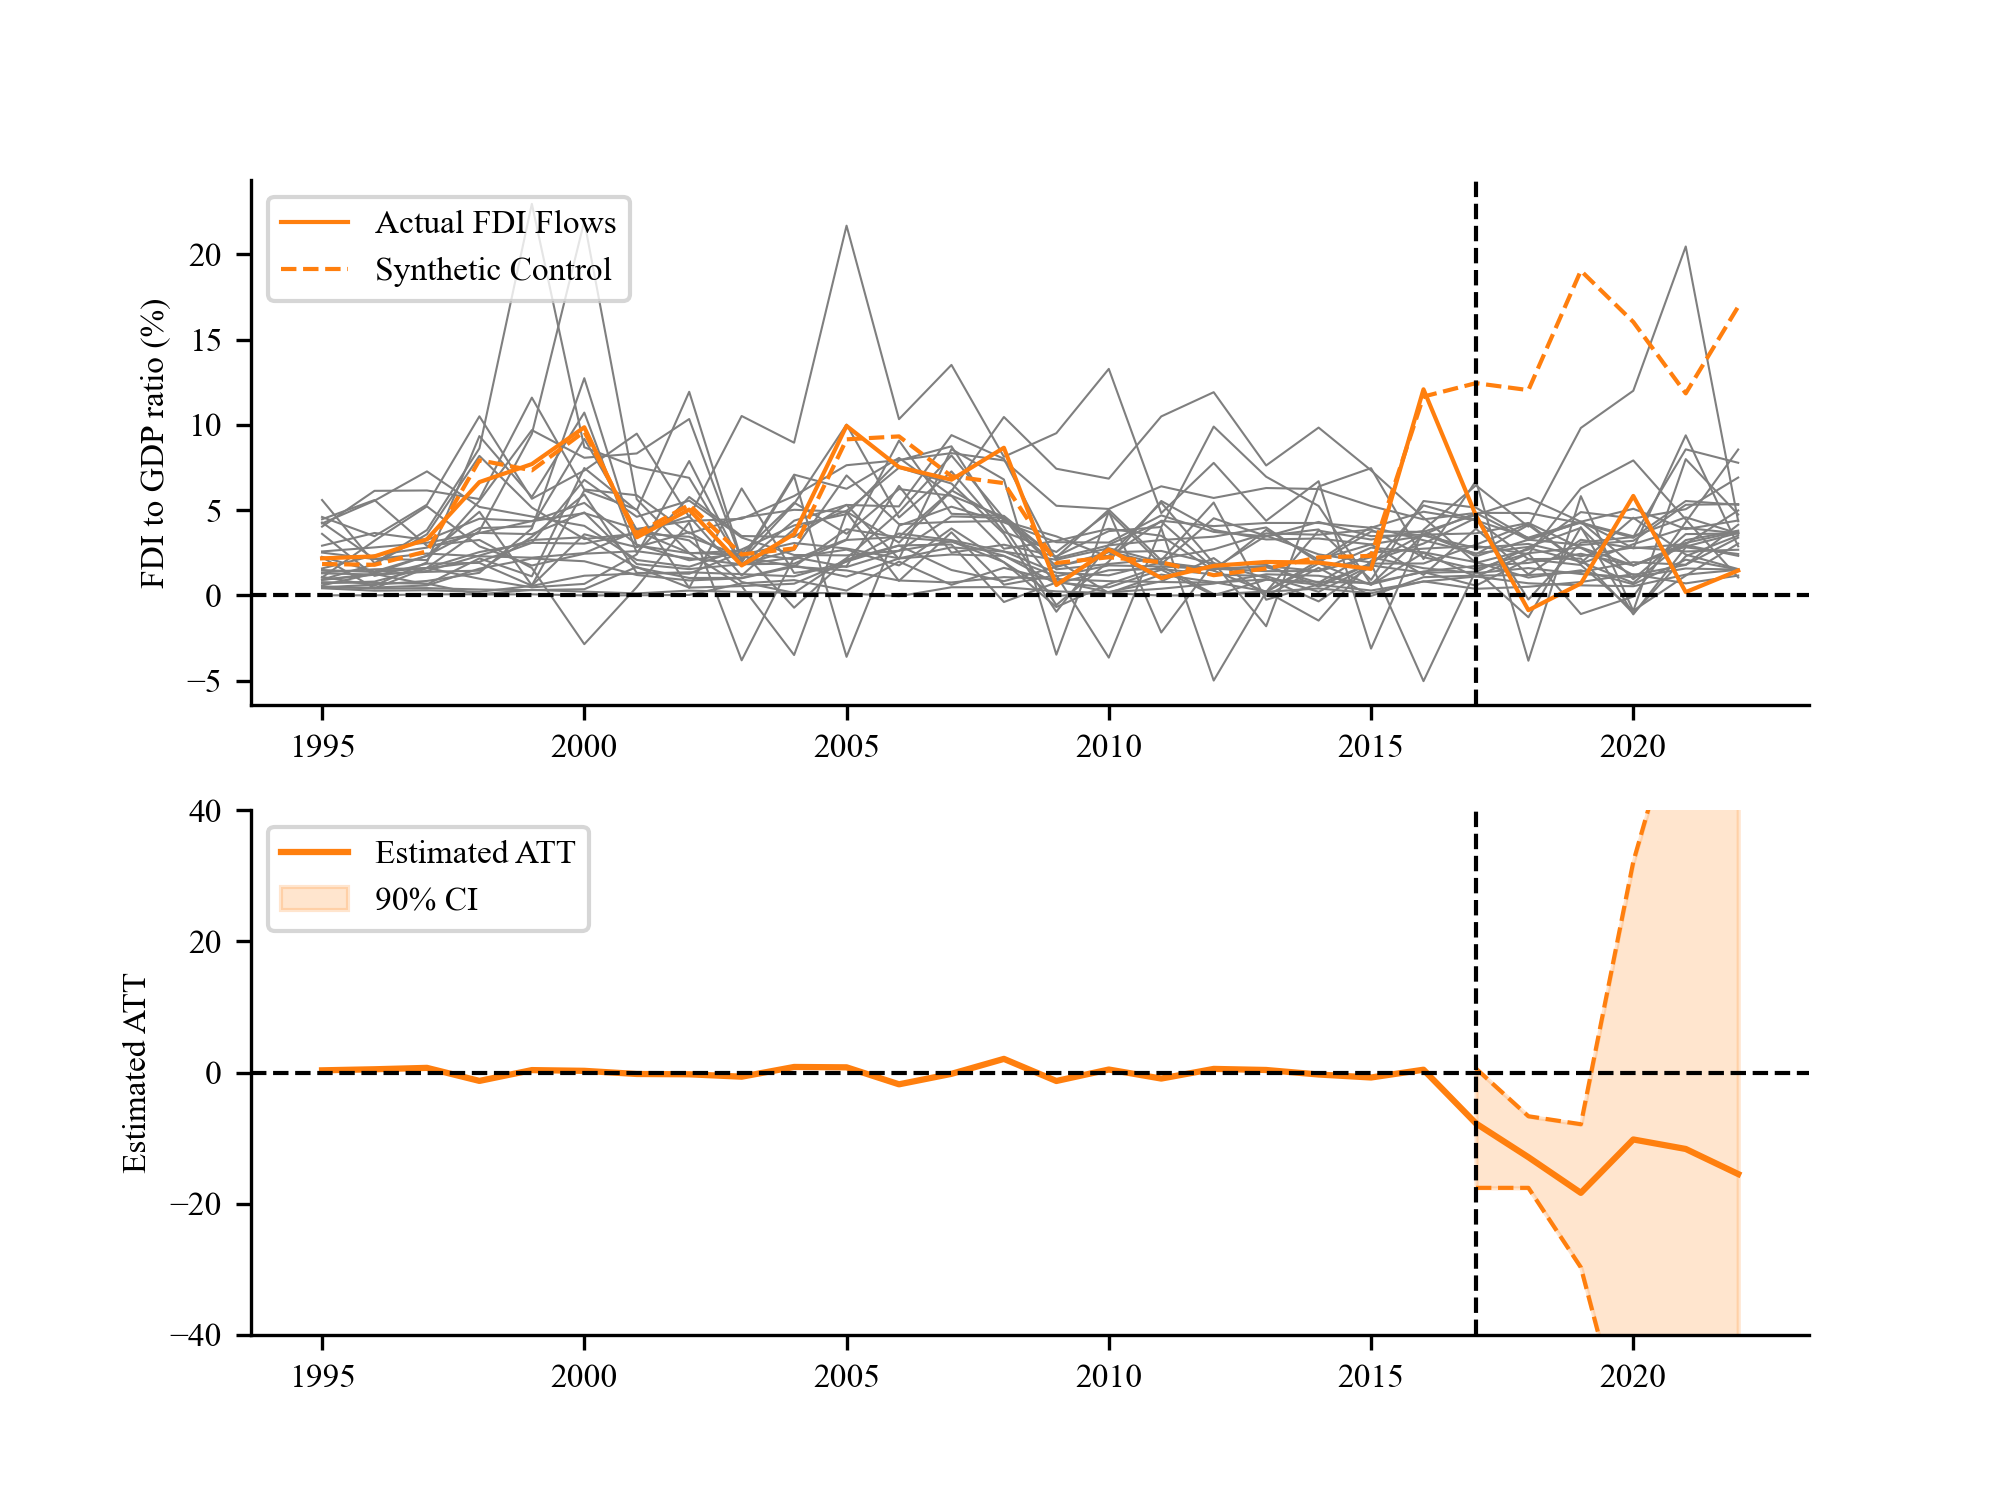
\includegraphics[scale=0.5]{figs/ukfdi_ipca.png}
\end{figure}
\end{frame}
\end{document}